\subsection{Experimental design}

\subsubsection{Conceptual basis}
Regular expression languages are infinite and exhibit substantial variety, but programmers are likely to use them for a limited number of purposes.  The goal of this study is to identify categories of regular expression usage and the frequency of usage in these categories so that designers of regular expression languages and end-user tools can better support what is most useful to programmers.  This study employs a sequence of two categorization attempts to achieve its goal.
\begin{itemize}\itemsep -1pt
\item[1] determine an objective behavioral similarity score for all pairs of regexes, and find clusters of highly similar regexes, so that a large number of regexes can be seen as a modest number of clusters, and then manually categorize these clusters
\item[2] using the categories from step 1 as a guide in understanding how behavior will cluster, create a categorization technique by iterative attempts and then manually categorize regexes based on inspection alone
\end{itemize}

\subsubsection{Implementation details for manual categorization}
The following categorization scheme was created after three visual scans of the top 3000 regexes (by number of projects), and eight iterative manual categorization passes over the top 130 regexes:

\paragraph{Commonly observed categories} In this work, regexes will belong to the first category in the ordered list described here (categories are greedy).  Very long regexes (over 100 chars long) are treated as their own category without further investigation (unless recognized very easily), because their behavior is significantly complex so as not to properly belong to any other category.  From behavioral clustering, it was determined that web-based, bracket-parsing and code-based categories cluster strongly.  For other regexes, the degree of freedom limits the clustering technique: regexes composed of long strings with very little abstraction are not free to cluster by conceptual category because their string matching behavior rarely overlaps.  Some regexes contain recognizable words but also contain substantial abstract sections, usually to parse a file or a line representing a row of data.  Some regular patterns like dates, phone numbers and emails don't contain words but have a recognizable form.  A large portion of regexes contain just one or two characters, or character classes that may be used for de-serialization or delimiter-based work, but are hard to guess the exact application for.  In these free-clustering regexes, anchors often make a big difference, and will be considered at the same time.  Finally, a few catch-all categories for regexes that are difficult to guess the application for are used.  The first category is questions, which have a regularity the purpose of which is hard to understand such as \cverb![a-f0-9]{40}!.  , vanilla, such as \cverb![^\w\s-]!, \cverb!\d+!, \cverb!! or \cverb!! which


\begin{itemize}
anchors are ignored for less free regexes

web based
\item[ t ] tags      scanning for known HTML tags like \cverb!<div>.*!
\item[ x ] xml       non-HTML tags usually composed of whole words or with attributes
\item[ w ] web       parsing urls, IP addresses and web protocols

zero freedom
\item[ . ] marooned      a single character
\item[ h ] hex           using \cverb!\x[a-f0-9][a-f0-9]! or similar

code based
\item[ = ] operator  recognize a line of code (has `=', `+' or operators) without capturing
\item[ m ] message     scanning for an expected message phrase, not just a keyword
\item[ k ] keyword   recognize code keywords like 'include' or `std::bitset' or functions like out.println() without operators
\item[ b ] brackets  capturing or matching all content within brackets like \cverb!<.*?>! or \cverb!<[^>]*?>!


non-free-clustering long strings - all on approximately the same level
\item[ g ] args       recognize a shell command (usually with arguments)
\item[ l ] label     finding a plain label like `LIST OF EDGES' or `WIN_UTILS'
\item[ f ] file       recognize a file path or filename with particular contents

mostly-free-clustering regular strings

\item[ d ] dates         parsing a simple string code like a date format
\item[ n ] numbers       parsing a phone number, ssn, numeric date, regular number
\item[ i ] identifier    identifiers (alphanumeric) with a restriction (must be capitol first, have a `@'), or dealing with word-default variants

free-clustering strings
anchored prefix for fre-clustering strings a, so \cverb!\s*! is s for `space', but \cverb!^\s*$! is `as' because of \cverb!^! and \cverb!$! (only needs one anchor to require an anchor prefix).
\item[ \\ ] backslash    dealing mostly with backslashes like \cverb!\\(.)! - easy to recognize because the pattern for this will contain four backslashes: \verb!"\\\\"!
\item[ s ] space         whitespace only

\item[ p ] punctuation   contains punctuation (not just slashes), maybe with whitespace like, \cverb!\s*,\s*!

catch-all (no anchor prefix)
\item[ L ] LONG        too long to deal with
\item[ q ] question    regular pattern but hard to identify
\item[ v ] vanilla     vanilla defaults and mixes, maybe punctuation but not as required, like \cverb![-\s]+!
\item[ y ] why?        does not do anything - no intent detectable



\todoMid{continue this intro}

\paragraph{Determining behavioral similarity} An ideal analysis of regex behavioral similarity would use subsumption or containment analysis. However, a tool that could facilitate an analysis of the corpus could not be found.  This is likely due to features like back-references, positional anchors and look-arounds that are ubiquitously excluded from the feature sets of regex analysis tools that are able to build automata and thereby perform containment analysis.  For this reason, a new technique using string matching was developed that can create a similarity score between two regexes with existing technology.

\begin{figure}[tb]
\centering
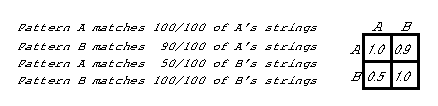
\includegraphics[height=0.6in]{nontex/illustrations/minimalMatrix.eps}
\caption{A similarity matrix created by counting strings matched}
\label{fig:minimalMatrix}
\end{figure}

\begin{figure}[tb]
\centering
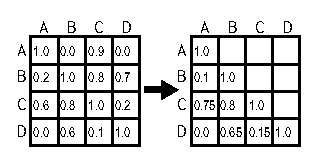
\includegraphics[width=0.7\columnwidth]{nontex/illustrations/matrixToGraph.eps}
\vspace{-6pt}
\caption{Creating a similarity graph from a similarity matrix}
\vspace{-6pt}
\label{fig:matrixToGraph}
\end{figure}



\subsubsection{Overview of process}

The similarity analysis used in this study clusters regular expressions by their behavioral similarity on matched strings.
Consider two unspecified patterns {\tt A} and {\tt B}, a set {\tt mA} of 100 strings that pattern {\tt A} matches, and a set {\tt mB} of 100 strings that pattern {\tt B} matches.
If pattern {\tt B} matches 90 of the 100 strings in the set {\tt mA}, then {\tt B} is 90\% similar to {\tt A}.
If pattern {\tt A} only matches 50 of the strings in {\tt mB}, then {\tt A} is 50\% similar to {\tt B}.
We use similarity scores to create a similarity matrix as shown in Figure~\ref{fig:minimalMatrix}.
In row {\tt A}, column {\tt B} we see that {\tt B} is 90\% similar to {\tt A}.
In row {\tt B}, column {\tt A}, we see that {\tt A} is 50\% similar to {\tt B}.  Each pattern is always 100\% similar to itself, by definition.

Once the similarity matrix is built, the values of cells reflected across the diagonal of the matrix are averaged to create a half-matrix of undirected similarity edges, as illustrated in Figure~\ref{fig:matrixToGraph}.
This facilitates clustering using the  Markov Clustering (MCL) algorithm\footurl{http://micans.org/mcl/}.
We chose MCL  because it offers a fast and tunable way to cluster items by similarity and it is particularly useful when the number of clusters is not known \emph{a priori}.


In the implementation, strings are generated for each pattern using Rex~\cite{rex}.  Rex generates matching strings by representing the regular expression as an automaton, and then passing that automation to a constraint solver that generates members for it\footurl{http://research.microsoft.com/en-us/projects/rex/}.  If the regex matches a finite set of strings smaller than 400, Rex will produce a list of all possible strings.
Our goal is to generate 400 strings for each pattern to balance the runtime of the similarity analysis with the precision of the similarity calculations.

For clustering, we prune the similarity matrix to retain all similarity values greater than or equal to 0.75, setting the rest to zero, and then using MCL.
This threshold was selected based on recommendations in the MCL manual. The impact of lowering the threshold would likely result  in either the same number of more diverse clusters, or a larger number of clusters, but is unlikely to markedly change the largest clusters or their summaries, which are the focus of our analysis for \todoMid{some research question reference}.
, but further study is needed to substantiate this claim.
We also note that MCL can also be tuned using many parameters, including inflation and filtering out all but the top-k edges for each node.
After exploring the quality of the clusters using various tuning parameter combinations, the best clusters (by inspection) were found using an inflation value of 1.8 and k=83.   The top 100 clusters are categorized by inspection into six categories of behavior.

The end result is clusters and categories of highly behaviorally similar regular expressions, though we note that this approach has a tendency to over-approximate the similarity of two regexes. We measure similarity based on a finite set of generated strings, but some regexes  match an infinite set (e.g., \verb!ab*c!), so measuring similarity based on the first 400 strings may lead to an artificially high similarity value. To mitigate this threat, we chose a large number of generated strings for each regex, but future work includes exploring other approaches to computing regex similarity.


